\documentclass[12pt]{article}
\title{\textbf{Perceptions \& Use of BitTorrent P2P File Sharing by Dartmouth College Students\footnote{This paper constitutes the final project for the Fall 2013 iteration of CS 55: Security and Privacy, taught by Charles C. Palmer, Adjunct Professor of Computer Science, Dartmouth College; CTO Security and Privacy, IBM Research.}}}
\author{Alex Gerstein\textsuperscript{1} and Scott Gladstone\textsuperscript{2} \\
	\\ \textsuperscript{1} Dartmouth College\\ Computer Science, Film Studies\\ \texttt{alex.gerstein@dartmouth.edu} 
	\and
	\textsuperscript{2} Dartmouth College\\ Computer Science, Economics\\ \texttt{scott.gladstone@dartmouth.edu}
}
\date{\today}

\usepackage[margin=1.0in]{geometry}
\setlength{\parskip}{10pt plus 1pt minus 1pt}
\usepackage{fancyhdr}
\usepackage{enumerate}
\usepackage{multicol}
\usepackage{fixltx2e}
\usepackage{graphicx}
\usepackage[font=small,labelfont=bf]{caption}
\usepackage[superscript,biblabel]{cite}

\begin{document}

\maketitle
\begin{abstract}
In our final project, we hope to investigate peer-to-peer (P2P) file sharing network protocols, specifically those related to torrenting (BitTorrent). After a general overview of the system and security flaws present, we plan to examine P2P in the context of Dartmouth College. By surveying students and speaking to Dartmouth College Computing Services, we hope to understand the disparity between the perception and actual use by students of torrent networks. If available, we also hope to obtain and analyze data from the College on student bandwidth habits, download frequencies, or other metrics that the College records. The outline below summarizes the questions we hope to answer and the individuals we hope to speak with.
\end{abstract}

\pagebreak
\section{Introduction}

BitTorrent is a protocol supporting peer-to-peer (P2P) file sharing that facilitates the distribution of large data files over the Internet \cite{BitTorrent}. BitTorrent is one of the most common protocols for transferring large files and is often used for distribution of very popular files and files available for free, such as literary texts, audio files, movies, and applications. ``Torrenting'' is the process by which a user engages with a BitTorrent client in order to send and receive those desired files. To understand the uniqueness -- and security implications -- of the BitTorrent protocol, one must first develop a working understanding of P2P file sharing. From there, the legal implications of P2P file sharing and BitTorrent can be made clear. With this foundation, the authors then describe a study in which data about student perceptions of torrenting at Dartmouth College are compared with data collected by Dartmouth College network administrators describing student incidences of torrenting. Conclusion and policy recommendations are then made with the goal of aligning student perceptions and administrative desires.

\subsection{Peer-to-Peer (P2P) File Sharing}
According to one Internet dictionary, P2P is a ``type of Internet network that allows users with the same program to connect with each other and access files on one another's hard drives without the intervention of a server computer,'' \cite{NYTimes}. This decentralized network architecture consists of individual nodes called \emph{peers} that act as both suppliers and consumers of resources. In P2P networks, tasks are shared among multiple, interconnected peers who each make a portion of their resources -- processing power, disk storage, or network bandwidth -- available to all network participants, without the centralized coordination of a server-client model \cite{scholl}. A comparison of a decentralized-P2P network and a centralized server-based network are presented in Figure 1 and Figure 2 below.

\begin{figure}[h!]
\centering
\begin{minipage}[b]{0.45\linewidth}
	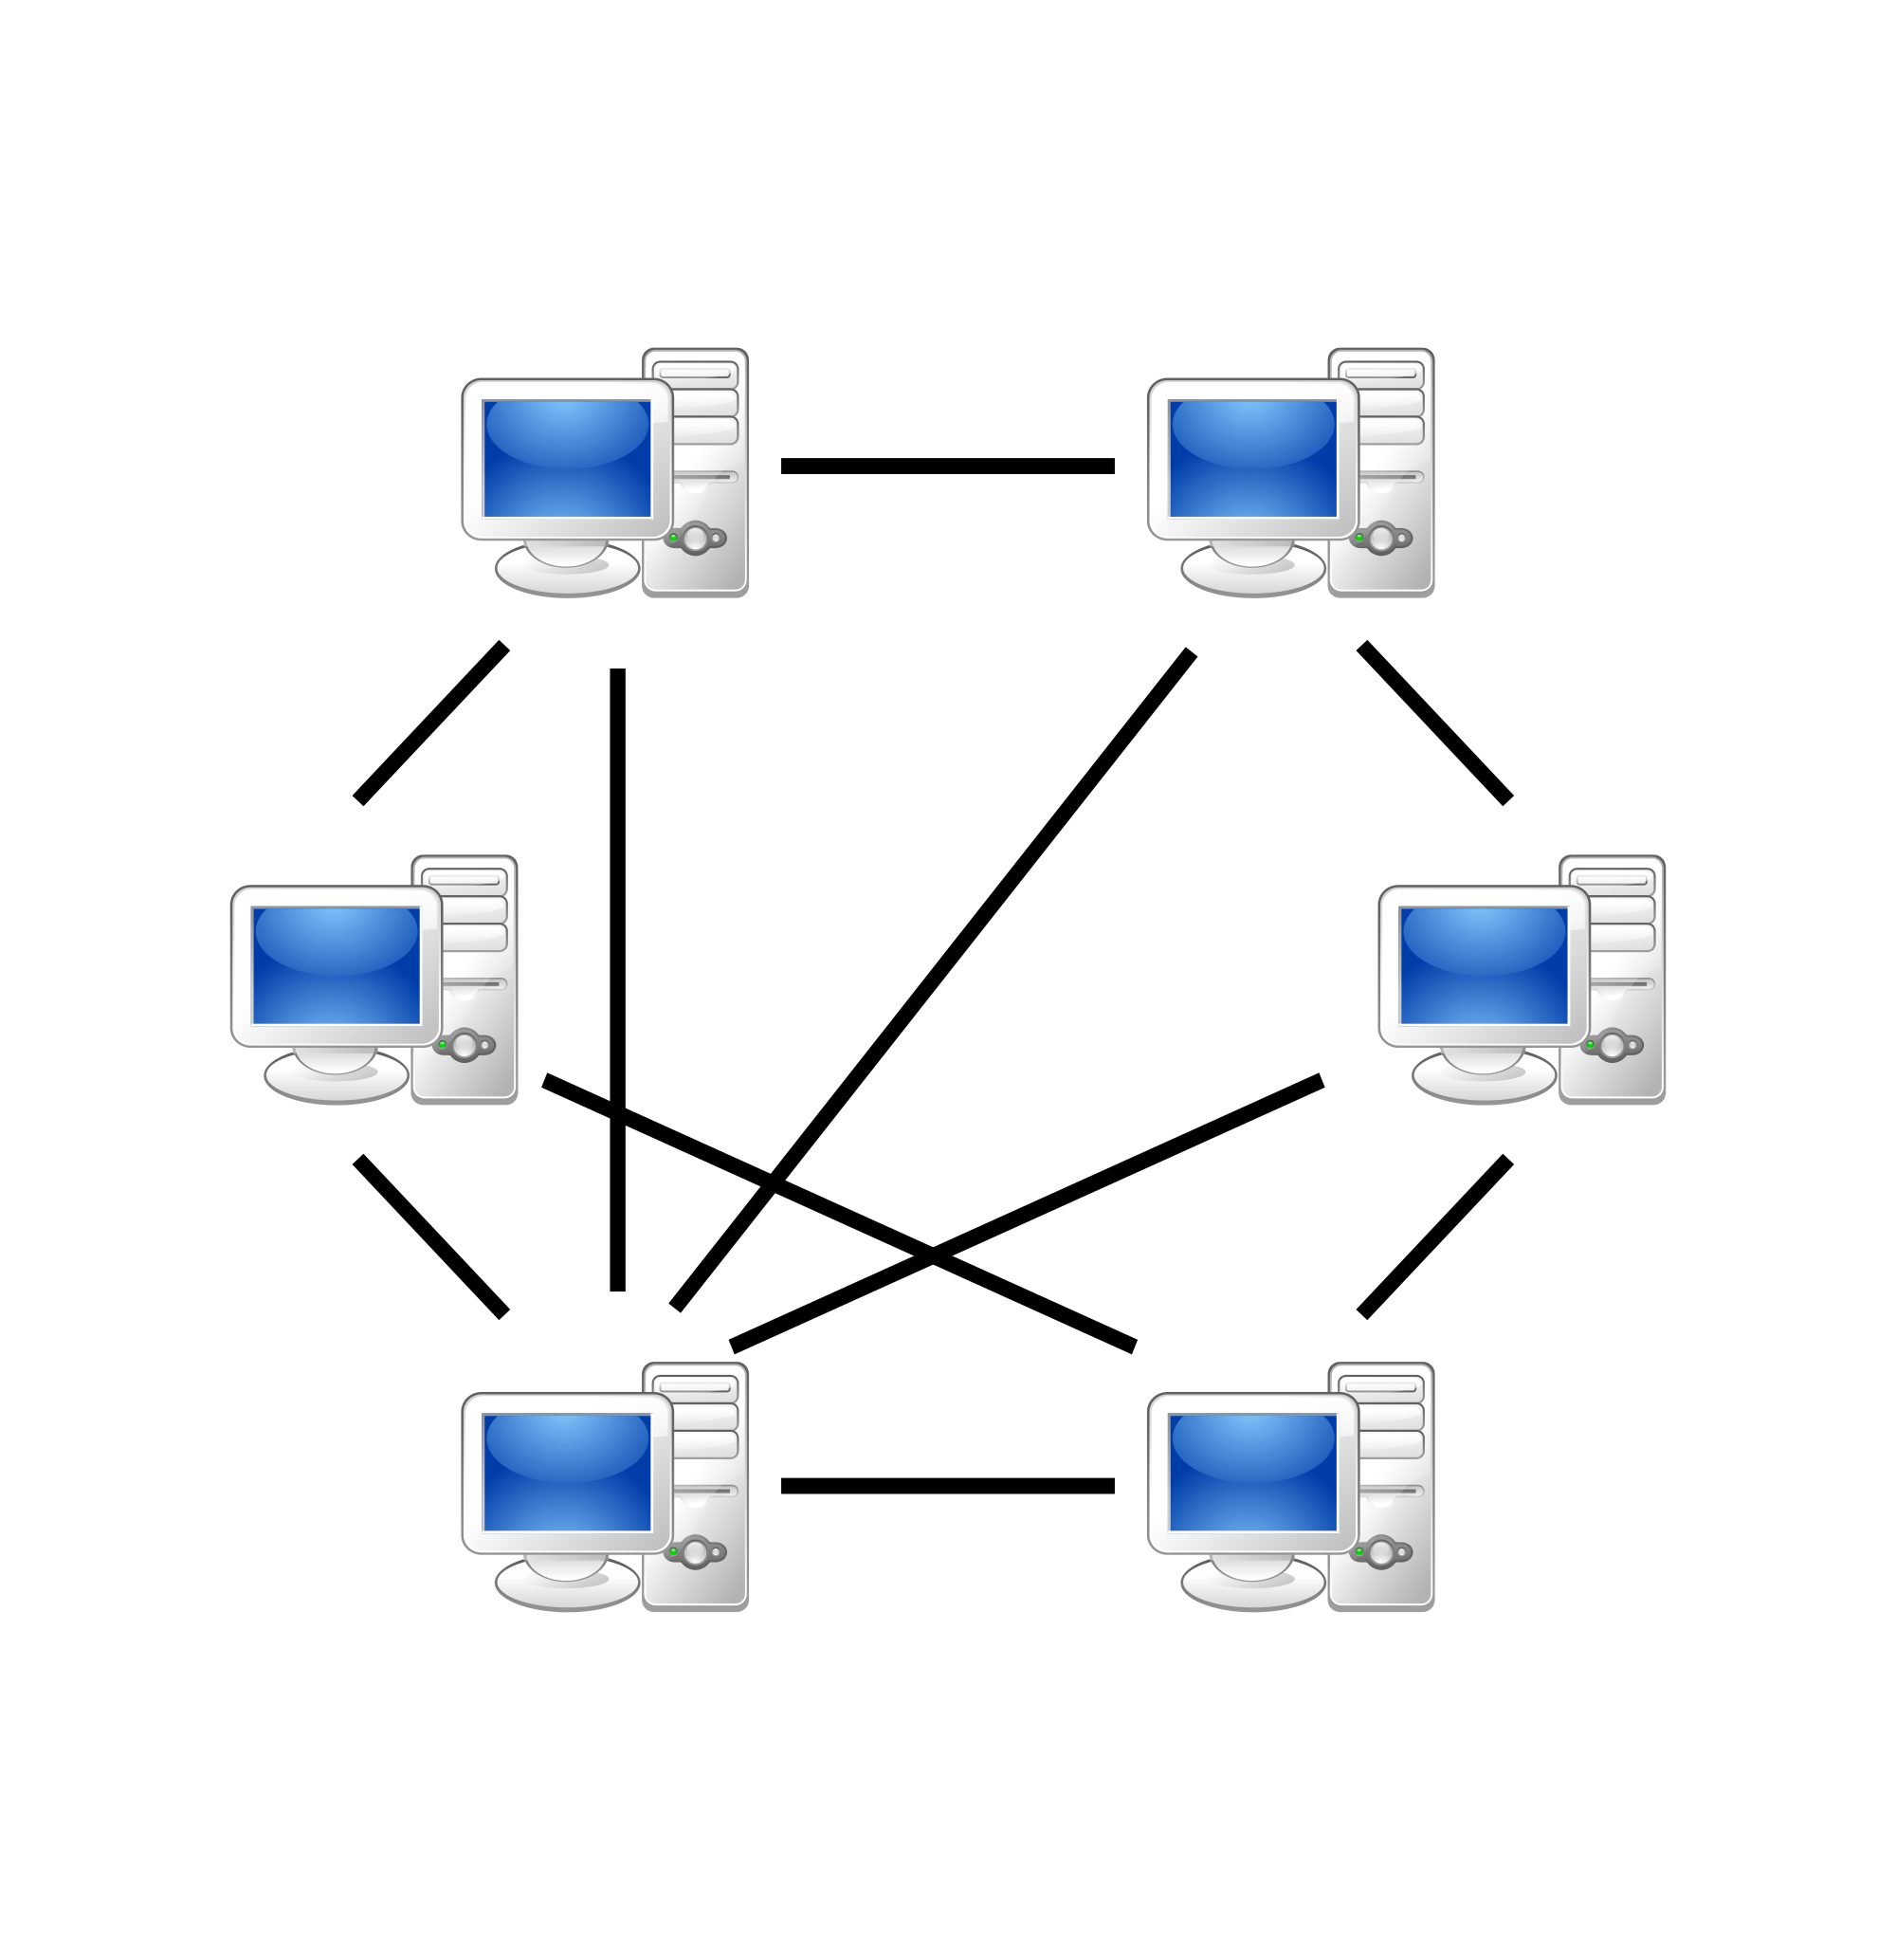
\includegraphics[width=56mm]{P2P-network}
	\caption{A peer-to-peer (P2P) network with interconnected nodes (``peers'') sharing resources. Source: Wikipedia.}
	\label{p2p_network}
\end{minipage}
\quad
\centering
\begin{minipage}[b]{0.45\linewidth}
	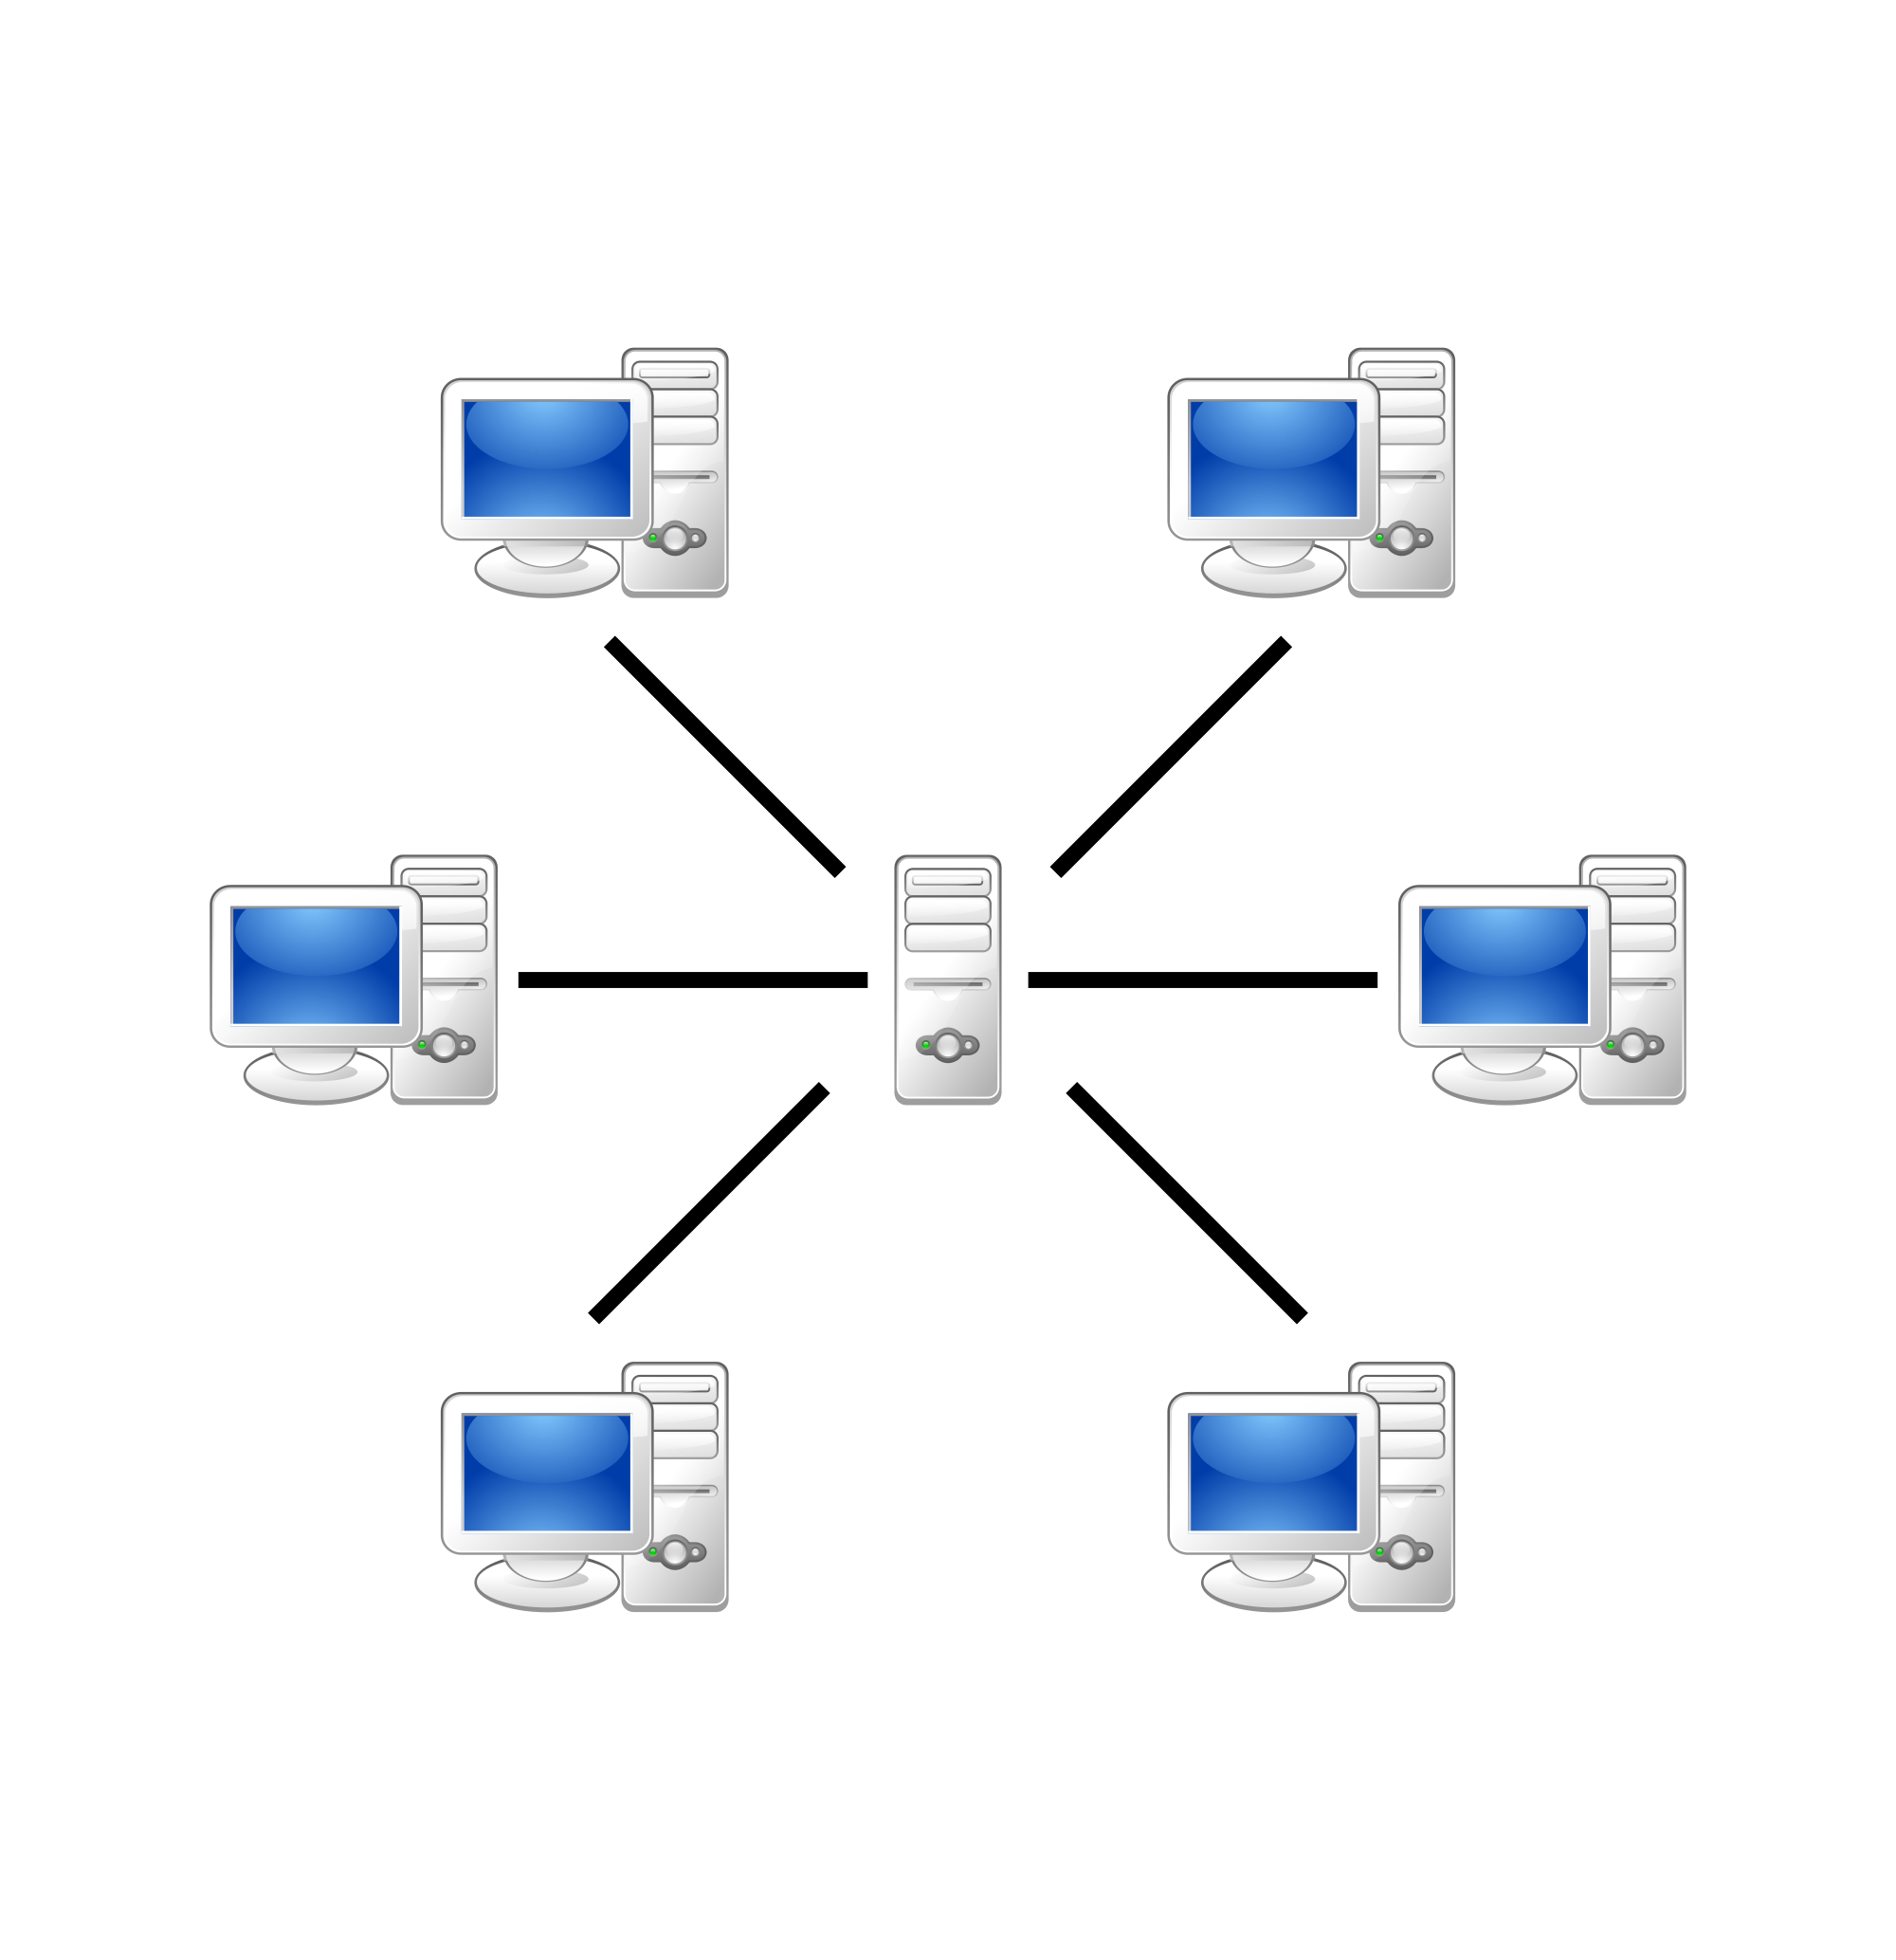
\includegraphics[width=56mm]{Server-based-network}
	\caption{A client-server model network, where individual clients request services from centralized servers. Source: Wikipedia.}
	\label{p2p_network}
\end{minipage}
\end{figure}

P2P networks are often found in residential home networks, allowing users to configure their computers in peer workgroups to allow sharing of files, printers, and other resources among all devices; with a number of computers running similar network protocols, P2P is a convenient way to access shared resources \cite{About}. However, the term ``P2P'' used today generally does not refer to the network architecture from which its name is derived, but to P2P file sharing systems. Using P2P software applications such as Napster or Kazaa, users are able to search for, transfer, and download data files over the Internet with any user on the same P2P file sharing network. The implications of such a system were huge: if \emph{any} user on the system had a file that another user demanded, the second user could -- via the network -- obtain the file. The second user would then also be a source of the file in the P2P network, making it faster and easier for more users to download the files. 

The first P2P file sharing networks, such as the purely-mp3 sharing network Napster, relied on a central index server to assist with the transfer of files. When someone searched for a file, the central index server -- which contained an index of all of the users and their shared content -- searched for all available copies of the file and presented them to the user; the file would then be transferred directly between the two private computers \cite{P2PFileSharewiki}. Because the file sharing occurred over a central network, Napster was held liable for copyright infringement over the sharing of mp3 files and was shut down in 2001 \cite{napster}. New protocols such as BitTorrent represent a technological evolution of P2P file sharing networks.

\subsection{BitTorrent Protocol}
What is BitTorrent (protocol)?
What makes BitTorrent different from other P2P systems?
What makes BitTorrent difficult to track?

\subsection{BitTorrent Security Concerns}
What are security issues related to using BitTorrent?

%%%%%%%%%%%%%%%%%%%%%%%
%%%%%%%%%%%%%%%%%%%%%%%

\section{Legal Issues}
Torrenting is not inherently illegal. 

\subsection{Copyright Law Violations}
What are the legal implications for an individual user for torrenting copyrighted information?

\subsection{Dartmouth College Copyright Policy}
What are the legal implications for a university like Dartmouth with students that do illegal torrenting?
What are some past cases and punishments relating to torrenting?

\pagebreak
\begin{thebibliography}{9}
\bibitem{BitTorrent} ``BitTorrent: Beginner's Guide.'' \emph{BitTorrent Inc.} Accessed November 4, 2013. Available at http://www.bittorrent.com/help/guides/beginners-guide.
\bibitem{NYTimes} Shannon, Victoria. ``The End User: P2P starts to mature.'' \emph{New York Times}. July 9, 2005. Available at http://www.nytimes.com/2005/07/08/technology/08iht-ptend09.html.
\bibitem{scholl} R�diger Schollmeier, A Definition of Peer-to-Peer Networking for the Classification of Peer-to-Peer Architectures and Applications, Proceedings of the First International Conference on Peer-to-Peer Computing, IEEE (2002).
\bibitem{About} http://compnetworking.about.com/od/p2ppeertopeer/a/p2pintroduction.htm
\bibitem{P2PFileSharewiki} ``Peer-to-peer file sharing.'' \emph{Wikipedia}. Accessed November 4, 2013. Available at http://en.wikipedia.org/wiki/Peer-to-peer\_file\_sharing\#History.
\bibitem{napster} Douglas, Guy. ``Copyright and Peer-To-Peer Music File Sharing: The Napster Case and the Argument Against Legislative Reform.'' \emph{Murdoch University Electronic Journal of Law.} Vol. 11, No. 1 (March 2004). Available at http://www.murdoch.edu.au/elaw/issues/v11n1/douglas111.html.
\end{thebibliography}

** statistics on P2P we may want to use: http://www.ipoque.com/sites/default/files/mediafiles/documents/internet-study-2008-2009.pdf

\end{document}
